
\documentclass[11pt,fleqn]{article} 
\usepackage[margin=0.8in, head=0.8in]{geometry} 
\usepackage{amsmath, amssymb, amsthm}
\usepackage{fancyhdr} 
\usepackage{palatino, url, multicol}
\usepackage{graphicx, pgfplots} 
\usepackage[all]{xy}
\usepackage{polynom} 
%\usepackage{pdfsync} %% I don't know why this messes up tabular column widths
\usepackage{enumerate}
\usepackage{framed}
\usepackage{setspace}
\usepackage{array,tikz,tabularx}
\usetikzlibrary{calc, patterns, shapes, arrows}

\pgfplotsset{compat=1.6}

\pgfplotsset{soldot/.style={color=black,only marks,mark=*}} \pgfplotsset{holdot/.style={color=black,fill=white,only marks,mark=*}}
\pgfplotsset{my style/.append style={axis x line=middle, axis y line=
middle, xlabel={$x$}, ylabel={$y$}, axis equal }}


\pagestyle{fancy} 
\lfoot{}
\rfoot{3-3 Derivative Rules}

\begin{document}
\renewcommand{\headrulewidth}{0pt}
\newcommand{\blank}[1]{\rule{#1}{0.75pt}}
\newcommand{\bc}{\begin{center}}
\newcommand{\ec}{\end{center}}
\renewcommand{\d}{\displaystyle}

\vspace*{-0.7in}

%%%%%%%%%intro page
\begin{center}
  \large
  \sc{Section 3-3: Derivative Rules}\\
\end{center}
\begin{enumerate}
\item Using what you know about the graphs of the functions below, determine their derivatives\\
	\begin{tabularx}{\textwidth}{XXXX}
	$f(x)=10$&$g(x)=x$&$h(x)=\pi x$&$j(x)=\pi x+1$\\
	&&&\\
	$f'(x)=\underline{\hspace{0.5in}}$&$g'(x)=\underline{\hspace{0.5in}}$&$h'(x)=\underline{\hspace{0.5in}}$&$j'(x)=\underline{\hspace{0.5in}}$\\
	\end{tabularx}
	
\item Use the definition of the derivative to find the derivatives for each of the following functions:
	\begin{enumerate}
	\item $f(x)=x^2$
	\vfill
	\item $f(x)=x^3$
	\vfill
	\end{enumerate}

\vfill
\item Recall the following results below:
\begin{tabular}{l || ll}
work& $f(x)$ &$f'(x)$\\
\hline
&&\\
(worksheet \S 3.1)\quad&$x^{-1}$\quad &$-1x^{-2}$\\
&&\\
(\S 3.1 \# 20) & $3x^{-2}$\quad & $-6x^{-3}$\\
&&\\
(\S 3.2 \#59)&$(\sqrt{2})x^{1/2}$\quad & $\frac{\sqrt{2}}{2}x^{-1/2}$\\
\end{tabular}
\vspace{.5in}

\item Use the data above to fill in the rules below. Assume $c$ and $n$ are fixed numbers.\\

\begin{tabularx}{\textwidth}{XXXX}
$\displaystyle\frac{d}{dx}\left[ c\right]=\underline{\hspace{0.5in}}$&
$\displaystyle\frac{d}{dx}\left[ x^n\right]=\underline{\hspace{0.5in}}$&
$\displaystyle\frac{d}{dx}\left[ x^n+c\right]=\underline{\hspace{0.5in}}$&
$\displaystyle\frac{d}{dx}\left[ cx^n\right]=\underline{\hspace{0.5in}}$
\end{tabularx}

\newpage
\item Use the graphs of $f(x)=\sin(x)$ and $g(x)=\cos(x)$ (below) to sketch the graph of their derivatives $f'(x)$ and $g'(x).$\\

{\Large{$f(x)=\sin(x)$}}\\
 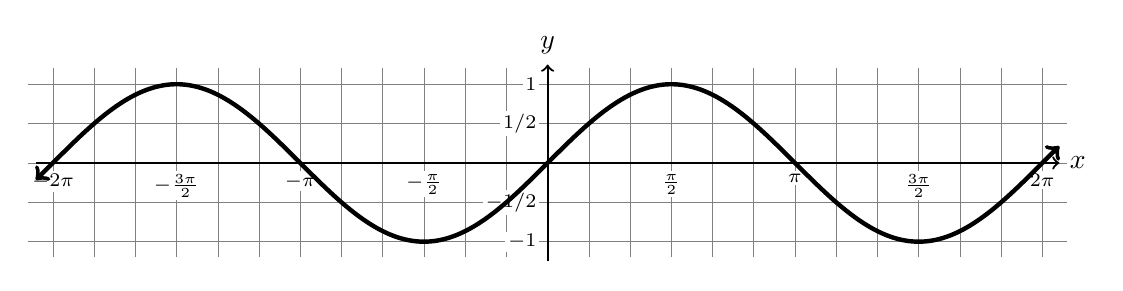
\begin{tikzpicture}[
tl/.style = {% tick labels
    fill=white, inner sep=1pt, font=\scriptsize,
            },
                        ]
% grid
\draw[gray, very thin, xstep=0.5235, ystep=0.5] (-6.6,-1.2) grid (6.6,1.2);
% y tick label
\foreach \y in {-1, -1/2, 1/2, 1}{\node[tl,left=1mm] at (0,\y) {$\y$};}
% x tick label
\foreach \x [count=\xx from -4] in 
       {-2\pi,          %-\frac{11\pi}{2}, -\frac{5\pi}{3},
        -\frac{3\pi}{2},%-\frac{4\pi}{3},  -\frac{7\pi}{6},
        -\pi,           %-\frac{5\pi}{6},  -\frac{2\pi}{3},
        -\frac{\pi}{2}, %-\frac{4\pi}{3},  -\frac{7\pi}{6},
        { },
         %\frac{\pi}{6},  \frac{\pi}{3},   
         \frac{\pi}{2},
         %\frac{2\pi}{3}, \frac{5\pi}{6},
         \pi,           %-\frac{7\pi}{6},   \frac{4\pi}{3},
         \frac{3\pi}{2}, %-\frac{5\pi}{3},  \frac{11\pi}{6},
         2\pi
        }{\node[tl,below=1mm] at (3*0.5235*\xx,0) {$\x$};}
% axes
    \draw[->,thick] (-6.5,0) -- (6.5,0) node[right] {$x$};
    \draw[->,thick] (0,-1.25) -- (0, 1.25) node[above] {$y$};
% curve
\draw[<->,ultra thick,
      domain=-6.5:6.5,samples=300,variable=\x] 
      plot (\x,{sin(deg{\x})});
    \end{tikzpicture}\\

{\Large{$g(x)=\cos(x)$}}\\
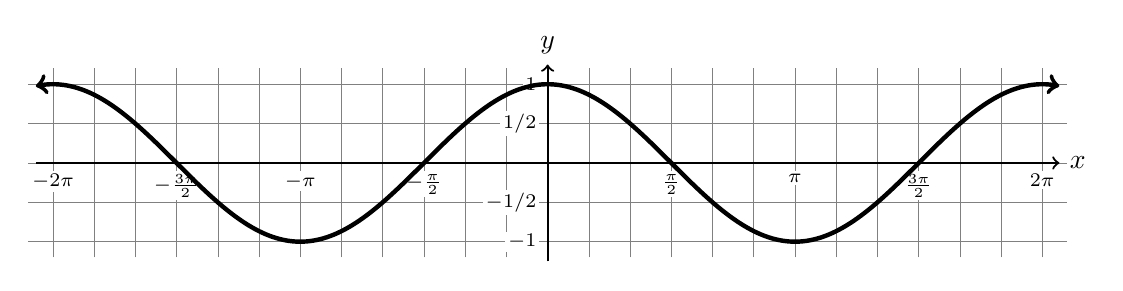
\begin{tikzpicture}[
tl/.style = {% tick labels
    fill=white, inner sep=1pt, font=\scriptsize,
            },
                        ]
% grid
\draw[gray, very thin, xstep=0.5235, ystep=0.5] (-6.6,-1.2) grid (6.6,1.2);
% y tick label
\foreach \y in {-1, -1/2, 1/2, 1}{\node[tl,left=1mm] at (0,\y) {$\y$};}
% x tick label
\foreach \x [count=\xx from -4] in 
       {-2\pi,          %-\frac{11\pi}{2}, -\frac{5\pi}{3},
        -\frac{3\pi}{2},%-\frac{4\pi}{3},  -\frac{7\pi}{6},
        -\pi,           %-\frac{5\pi}{6},  -\frac{2\pi}{3},
        -\frac{\pi}{2}, %-\frac{4\pi}{3},  -\frac{7\pi}{6},
        { },
         %\frac{\pi}{6},  \frac{\pi}{3},   
         \frac{\pi}{2},
         %\frac{2\pi}{3}, \frac{5\pi}{6},
         \pi,           %-\frac{7\pi}{6},   \frac{4\pi}{3},
         \frac{3\pi}{2}, %-\frac{5\pi}{3},  \frac{11\pi}{6},
         2\pi
        }{\node[tl,below=1mm] at (3*0.5235*\xx,0) {$\x$};}
% axes
    \draw[->,thick] (-6.5,0) -- (6.5,0) node[right] {$x$};
    \draw[->,thick] (0,-1.25) -- (0, 1.25) node[above] {$y$};
% curve
\draw[<->,ultra thick,
      domain=-6.5:6.5,samples=300,variable=\x] 
      plot (\x,{cos(deg{\x})});
    \end{tikzpicture} 



 \item Base on the work above, guess answers:  \begin{tabular}{ll}
	$\displaystyle\frac{d}{dx}\left[\sin(x) \right]=\underline{\hspace{0.5in}}$&
	$\frac{d}{dx}\left[ \cos(x) \right]=\underline{\hspace{0.5in}}$
	\end{tabular}

\item Four Big Rules\\
	 \begin{enumerate}
 	\begin{multicols}{2}
	\item Constant Multiple
	\item Sum (and Difference)
	\end{multicols}
	\vspace{1.5in}
	% \begin{multicols}{2}
	\item Product
	\vfill
	\item Quotient
	%\end{multicols}
	\vfill
	\end{enumerate}
\end{enumerate}
\end{document}
\end{multicols} 
\end{enumerate}
  \end{document}
\newpage
\item Use your intuition to evaluate the derivatives of the functions below and \emph{ask yourself what assumptions you are making.}
\begin{multicols}{2}
 \begin{enumerate}
\item $S(x)=x^5+\sin(x)$
\item $M(x)=20 \cos(x)$
\end{enumerate}
\end{multicols}
\vspace{1in}
\item Summary Rules


 \begin{enumerate}
 \begin{multicols}{2}
\item Sum and Difference
\item Constant Multiple
\end{multicols}
\vspace{1in}
 \begin{multicols}{2}
\item Product
\item Quotient
\end{multicols}
\vspace{1in}
\end{enumerate}

\item Find the derivatives of the functions below.
\begin{enumerate}
 \begin{multicols}{2}
\item $K(\theta) = \theta^{1/3} \sin(\theta)$
\item $j(x)=\frac{\cos(x) + \sqrt{2}}{x+1}$
\end{multicols}
\vspace{1in}
\end{enumerate}
\end{enumerate}
\end{document}
\item Use the definition to find the derivative of $H(x)=x^2.$\\
\vspace{2in}
\item If $f(x)=10,$ what should $f'(x)$ be and why? 
\vfill

\item If $f(x)=c,$ where $c$ is some real number, what is $f'(x)$? 
\vfill
\newpage
\item If $f(x)=x,$ what should $f'(x)$ be and why? 

\vfill
\item What about $f(x)=5x$? Explain.
\vfill
\item What about $f(x)=5x+10$? Explain.
\vfill

\item In the 3.2 notes on the definition of the derivative, we found that if $f(x) =\sqrt{x+5}=(x+5)^{1/2}$, then its derivative was: \\

Use this to determine the derivative of $g(x)=\sqrt{x}.$
\vfill
\item The Power Rule\\
\vfill
\item The Sum (and Difference) Rule\\
\vfill

\item The Constant Multiple Rule\\
\vfill

\newpage
\item Apply the rules to find the derivatives of the functions below. Simplify your answers and write with positive exponents.
	\begin{enumerate}
	\item $\displaystyle{f(x)=e^3}$\\
	\vfill

	\item $\displaystyle{f(x)=x^{-4}}$\\
		\vfill

	\item $\displaystyle{H(x)=4x^{3/2}+ 15}$\\
	\vfill

	\item $\displaystyle{j(x)=\frac{\sqrt{2}}{2}+x-8x^{2.3}}$\\
	\vfill

	\end{enumerate}
\item Find examples of $f(x)$ and $g(x)$ that demonstrate that the rules below are WRONG.\\
\begin{quote} INCORRECT: If $H(x)=f(x)g(x)$, then $H'(x)=f'(x)g'(x).$ \end{quote}
\vfill

\begin{quote} INCORRECT: If $H(x)=\frac{f(x)}{g(x)}$, then $H'(x)=\frac{f'(x)}{g'(x)}.$ \end{quote}
\vfill

\newpage
\item Product Rule  $\displaystyle{\frac{d}{dx}\left[f(x)\: g(x)\right]=}$\\
\vspace{.7in}

\item Example: Find the derivative of $f(x)=x^2\sin(x)$
\vfill
\item Quotient Rule: $\displaystyle{\frac{d}{dx}\left[\frac{f(x)}{g(x)}\right]=}$\\
\vspace{.7in}

\item Example: Use the Quotient Rule to find the derivative of $g(t)=\frac{\cos(t)}{1-2t}.$
\vfill
\item Notation\\
\vspace{.7in}
\item Higher Order Derivatives
\vspace{.7in}
\end{enumerate}
\end{document}	
